\subsubsection{VLAN de~\nameref{itm:vlan10}}
\par En una primera instancia, el primer resultado visible que se puede obtener es la
entrop\'ia de ambas fuentes de datos:

\begin{table}[!h]
\centering
  \begin{tabular}{c c}
    Fuente de Datos & Entrop\'ia \\
    \hline\hline
    Direcci\'on Origen & 3.87546 \\
    Direcci\'on Destino & 6.50272 \\
    \hline\hline
    \#IPs de las Fuentes & 4\,428\\
    \#Paquetes Capturados & 825\,978\\
    \hline
    \end{tabular}
  \bigskip
  \caption{Entrop\'ia VLAN \nameref{itm:vlan10}}
\end{table}

\par Hasta el momento, s\'olo con este \'unico dato, mucho no se puede decir sobre la red.
Pasaremos entonces analizar cada fuente por separada:


\subsubsection*{\underline{VLAN \nameref{itm:vlan10}: Fuente Origen}}\label{subsubsec:vlan10_src}

\begin{figure}[!ht]
    \centering
    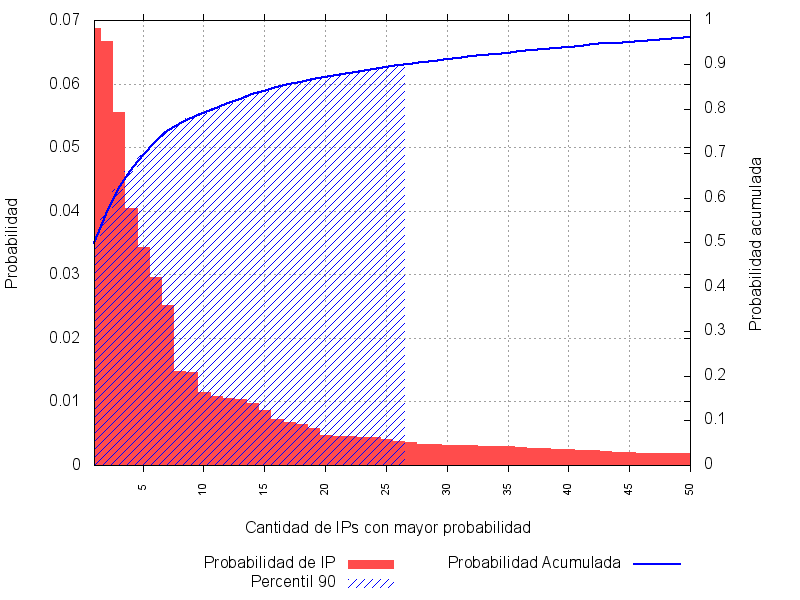
\includegraphics[width=0.5\textwidth]{escenario_1/vlan10/vlan10_src_bars_percentile90}
    \caption{Probabilidades VLAN \nameref{itm:vlan10} - Fuente Origen}
    \label{fig:vlan10_src_prob_per90}
\end{figure}

\par Observemos la figura \ref{fig:vlan10_src_prob_per90}. La misma se compone de 2
datos analizados sobre los resultados obtenidos. Por 
un lado, en el eje \textit{x} se tienen ordenadas, de mayor a menor, todas las IPs de la
fuente de datos seg\'un su probabilidad muestral. Los s\'imbolos en cuesti\'on (IPs) no
son expuestos en la gr\'afica a\'un ya que se solapar\'ian y har\'ian ilegible al gr\'afico.
En lugar de ello se expuso la cantidad de IPs que hay hasta cada punto marcado del eje%
\footnote{Donde dice \textit{5, 10, 15...}, se tienen de izquierda a derecha 5 IPs, 10
IPs, etc.}. 

\par En rojo tenemos la probabilidad muestral de los s\'imbolos (que por el orden impuesto
ir\'a obviamente decreciendo).

\par Por \'ultimo, en azul se puede ver la l\'inea de progreso de probabilidad acumulada.
En cada s\'imbolo del eje \textit{x}, la l\'inea azul nos indica cual es la sumatoria de
las probabilidades de todos los s\'imbolos (comenzando por el de mayor probabilidad) hasta
dicho punto.\\

\par As\'i pues, podemos observar que se llega al percentil 90 con tan solo los 27 s\'imbolos
de mayor probabilidad de la fuente. Es decir que menos del 0.01\% de los s\'imbolos aparecen
en nuestra fuente de datos con un 90\% de probabilidad.

\par Visto esto, ya nos interesa pasar a analizar de que IPs exactamente estamos hablando.
Como se vi\'o, en el an\'alisis lo m\'as determinante parecer\'ia ser aquellas IPs inclu\'idas
dentro del percentil 90. Las mismas se presentan a continuaci\'on:

\begin{figure}[!ht]
    \centering
    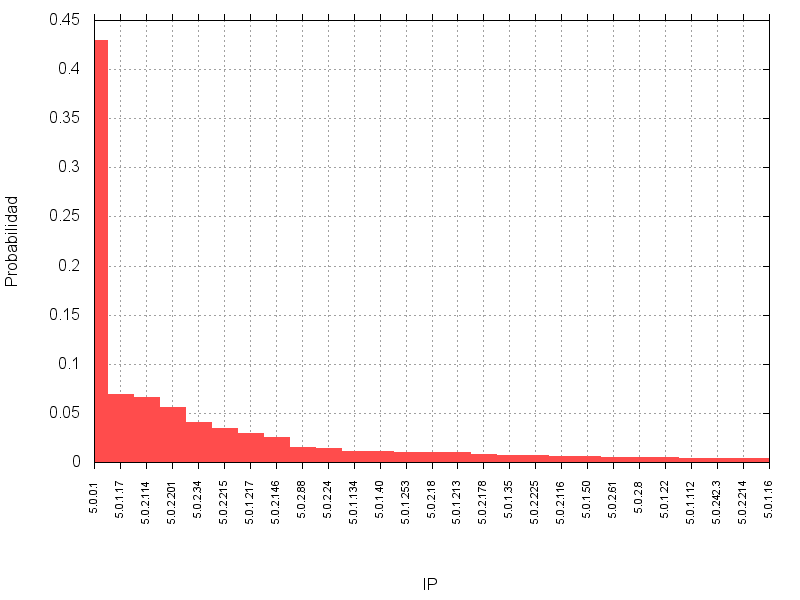
\includegraphics[width=0.5\textwidth]{escenario_1/vlan10/vlan10_src_probabilities_with_labels}
    \caption{IPs VLAN \nameref{itm:vlan10} - Fuente Origen}
    \label{fig:vlan10_src_prob_ips}
\end{figure}

\par Se puede observar en la figura \ref{fig:vlan10_src_prob_ips} que las primeras 6 IPs parecer\'ian
ser las principales de la red en enviar paquetes ARP (recordemos que estamos viendo los resultados
de la fuente de origen, es decir, los paquetes ARP cuya direcci\'on origen es la que fue
analizanda). Claramente estas IPs ya son candidatas a tener en cuenta al buscar nodos importantes
de nuestra red, ya que claramente est\'an env\'iando m\'as paquetes ARP que el resto, aunque el
motivo nos sea desconocido.


\subsubsection*{\underline{VLAN \nameref{itm:vlan10}: Fuente Destino}}\label{subsubsec:vlan10_dst}
\par Pasamos ahora a visualizar en la figura \ref{fig:vlan10_dst_prob_per90} los datos obtenidos
en la misma red, pero en la fuente destino, es decir, las IP's a las que fueron enviados los
paquetes ARP (o, dicho de otra forma, aquellos nodos a cuyos paquetes estaban destinados).

\begin{figure}[!ht]
    \centering
    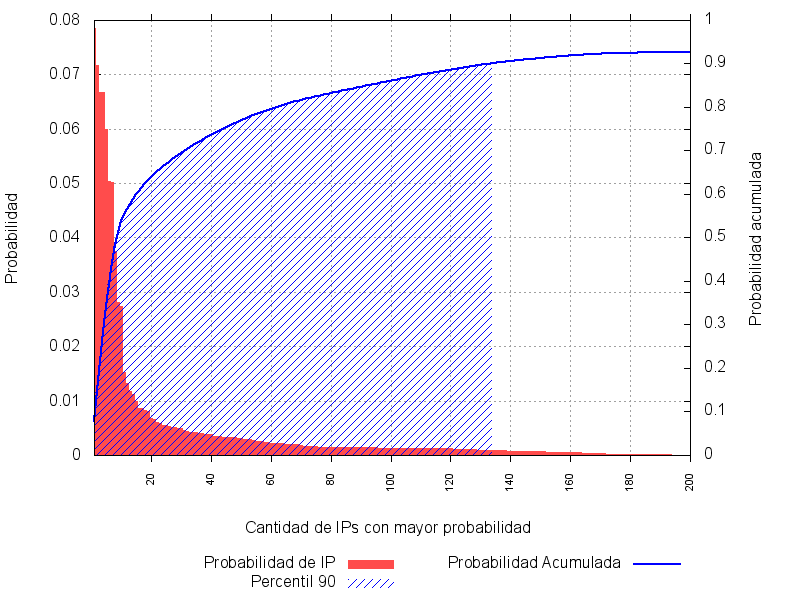
\includegraphics[width=0.5\textwidth]{escenario_1/vlan10/vlan10_dst_bars_percentile90}
    \caption{Probabilidades VLAN \nameref{itm:vlan10} - Fuente Destino}
    \label{fig:vlan10_dst_prob_per90}
\end{figure}

\par Nuevamente, se puede observar que se alcanza el percentil 90 de probabilidad de la
fuente con tan solo poco menos de 135 s\'imbolos (apr\'oximadamente representan un
0.03\% de la totalidad de IPs observadas en la fuente). Claramente, nos encontramos
nuevamente ante la situaci\'on de una red donde los destinos de los paquetes ARP
est\'an concentrados en unos pocos nodos. De hecho, no es casualidad que la cantidad
de personas que trabajan en esta red sean 70\footnote{Apr\'oximadamente}. Si se tienen
en cuenta algunos otras IPs que claramente no son de usuarios (posiblemente servidores)
y la posibilidad de usuarios con m\'as de una IP en la red\footnote{Interfases virtuales,
recordar que los \textit{hosts} de esta red son personal de un datacenter.}.

\par De hecho, si se observa con atenci\'on se podr\'a ver que en realidad, las primeras
50 IPs con mayor probabilidad conforman el percentil 80.

\par Observemos entonces, cuales son est\'as IPs que concentran la gran mayor\'ia
de la informaci\'on de nuestra fuente destino\footnote{En lugar de exponer la probabilidad
de las 135 IPs que componen el percentil 90, se tuvieron en cuenta las primeras 50 -percentil
80- dado que graficar tantos s\'imbolos har\'ia ilegible el gr\'afico y, a\'un m\'as importante
a\'un, a la hora de distinguir nodos importantes de la red, es muy probable que estos
se encuentren dentro de este percentil 80 que concentra tanta informaci\'on.}. Dicha informaci\'on
se presenta en la figura \ref{fig:vlan10_dst_prob_ips}.

\begin{figure}[!ht]
    \centering
    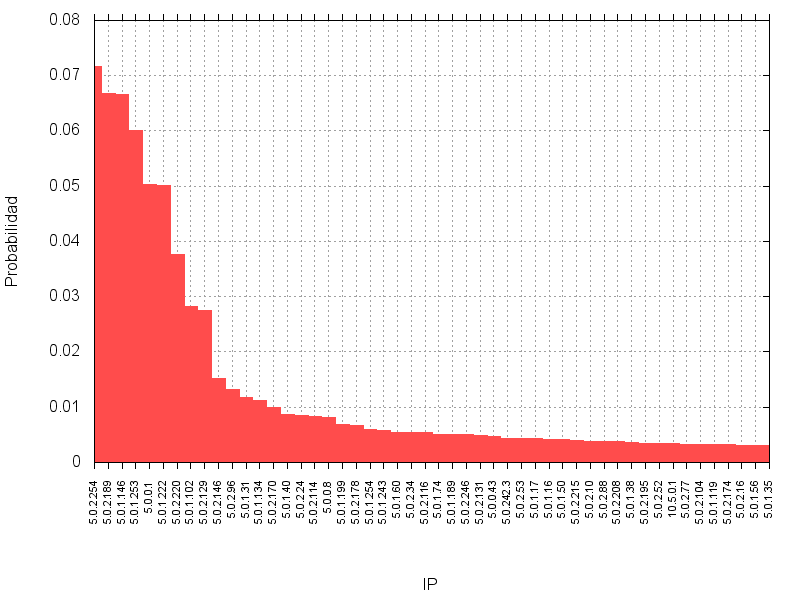
\includegraphics[width=0.5\textwidth]{escenario_1/vlan10/vlan10_dst_probabilities_with_labels}
    \caption{IPs VLAN \nameref{itm:vlan10} - Fuente Destino}
    \label{fig:vlan10_dst_prob_ips}
\end{figure}

\par En este \'ultimo gr\'afico podemos observar que dentro de las IPs que forman el percentil 80,
las 10 primeras IPs claramente componen la parte m\'as importante de la fuente. Es abrupta
la diferencia de las probabilidades, como se puede observar. As\'i pues, est\'as IPs que 
pareciesen ser muy solicitadas dentro de nuestra red, son claras candidatas a representar
nodos importantes.


\subsubsection*{\underline{VLAN \nameref{itm:vlan10}: Ambas Fuentes}}\label{subsubsec:vlan10_src_dst}
\par Toda la informaci\'on presentada hasta el momento nos permiti\'o identificar ciertas IPs
de la red (o s\'imbolos de la fuente) que seguramente son candidatos a representar algo notorio
o importante en la red \textit{sniffeada}. Pero a\'un no podemos llegar a conclusiones de la red,
dado que s\'olo obtivimos posibles IPs para dos fuentes distintas.

\par Para poder llegar a razonamientos coherentes sobre la red, debemos poder unir la informaci\'on
hasta ahora presentada de alguna manera. En primer instancia, es interesante observar las
relaciones entre las concentraciones de nodos de ambas fuentes (cantidad de IPs dentro del percentil
90/80 respecto de la totalidad de IPs de las fuentes) y las entrop\'ias:

\begin{table}[!h]
\centering
  \begin{tabular}{c c c c}
    Fuente& 
    Entrop\'ia & \begin{tabular}{@{}c@{}}Concentraci\'on \\ Percentil 90\end{tabular} 
    & \begin{tabular}{@{}c@{}}Concentraci\'on \\ Percentil 80\end{tabular}\\
    \hline\hline
    Origen & 3.87546 & 0.006\% & 0.002\%\\
    Destino & 6.50272 & 0.03\% & 0.015\%\\
    \hline\hline
    \end{tabular}
  \bigskip
  \caption{Concentraci\'on VLAN \nameref{itm:vlan10}}
  \label{tab:vlan10_concentracion}
\end{table}

\par Interesante como se ve el cuadro \ref{tab:vlan10_concentracion}, la \'unica nueva informaci\'on
que nos da es que claramente es que la incertidumbre de la fuente destino es mayor que la de la 
fuente destino. Es decir, mirando la concentraci\'on de los percentiles vemos que el 90\% de
probabilidades de la fuente destinoest\'a acumulado en un 0.03\% de los s\'imbolos de la fuente,
mientras que en la fuente origen est\'a a\'un m\'as concentrada. Esta concentraci\'on a nosotros,
dado nuestro objetivo, nos resulta \'util ya que nos permite reducir la cantidad de IPs que
probablemente cumplan con un rol importante dentro de la red.

\par As\'i pues llegamos a esta instancia con una reducci\'on de unas 160 IPs (entre ambas fuentes)%
\footnote{Se filtraron las IPs que componen los percentiles 90 de ambas fuentes.}
entre las cuales seguramente se encuentren los hosts importantes de la red \textit{sniffeada}. Se
presenta entonces a continuaci\'on un digrafo de la red entera, se\~nalando estas IPs candidatas.

\par Dado el gran tama\~no del \textit{dataset} (muchos nodos y muy denso en ejes\footnote{%
aproximadamente unos 4400 nodos con 12000 ejes}), se decidi\'o filtrar un poco m\'as los datasets
con alg\'un concepto intuitivo: si durante 77 horas de captura, un cierto par ordenado de direcciones
IP de un paquete ARP no se captur\'o m\'as de 500 veces, podemos asumir que dicho par no aporta
mucha informaci\'on, ya que se trata de informaci\'on espor\'adica que nos dan las fuentes de
datos.

\begin{figure*}[!t]
    \centering
    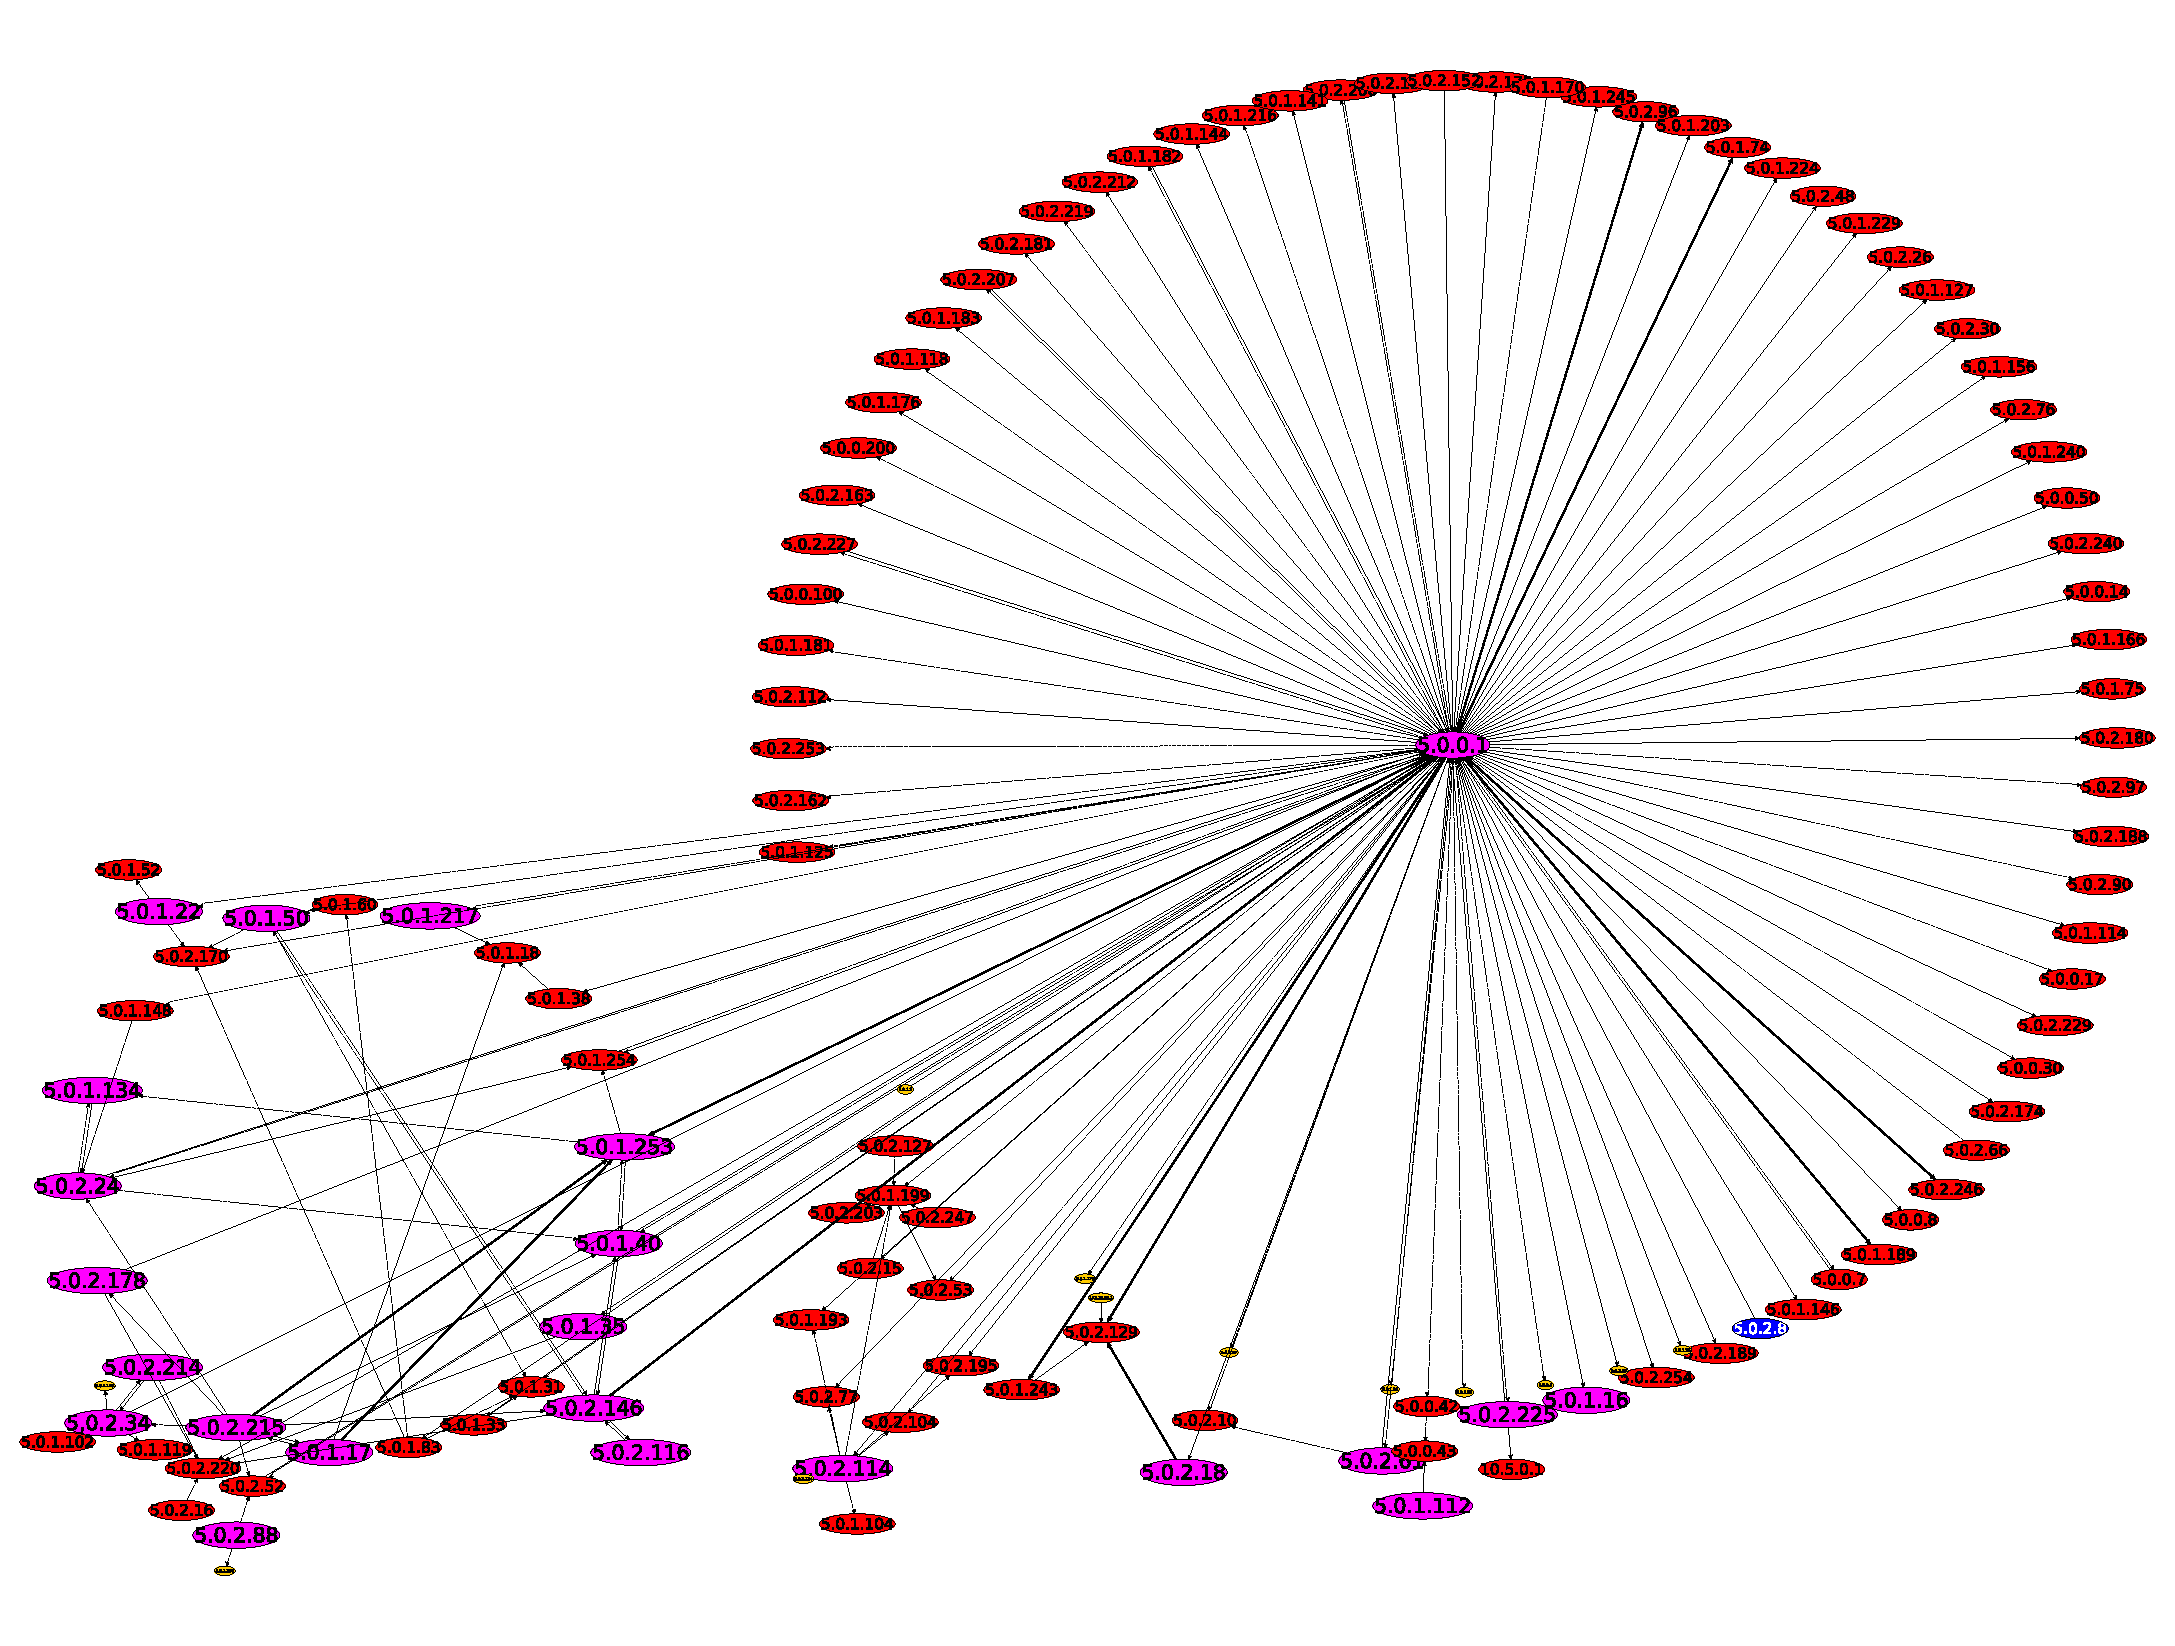
\includegraphics[width=\textwidth]{img/graph/escenario_1/vlan10/vlan10_500toEnd}
    \caption{Grafo VLAN \nameref{itm:vlan10}}
    \label{fig:vlan10_grafo}
\end{figure*}

\par En el grafo en cuesti\'on (figura \ref{fig:vlan10_grafo}) se colorearon los nodos
siguiendo la siguiente l\'ogica:

\begin{LaTeXdescription}
    \item[Rojo] Son los nodos que forman parte del percentil 90 de la fuente de
    direcciones de destino.\\

    \item[Azul] Son los nodos que forman parte del percentil 90 de la fuente de 
    direcciones de origen.\\

    \item[Violeta] Son las direcciones que forman parte del percentil 90 de ambas
    fuentes de direcciones.\\

\item[Ejes] Los ejes fuero formateados de manera tal que representacen el peso de los
    ejes. Es decir, la cantidad de paquetes con las direcciones origen y destino (o nodos)
    conectados por cada eje. A menor peso, la l\'inea ser\'a menos gruesa y hasta
    punteada, mientras que en el caso contrar\'i el eje ir\'a ganado grosor.\\

\end{LaTeXdescription}

\par Como se observa, el grafo parece indicar un flujo de paquetes ARP amplio desde
el nodo del centro hacia la gran mayor\'ia de los dem\'as nodos. En dicho nodo (que se
ampl\'ia en la figura \ref{fig:vlan10_grafo_centro}), puede notarse una afluencia
balanceada en cuanto a flechas entrando (direcci\'on destino) y flechas saliendo
(direcci\'on origen\footnote{No por nada dicha IP est\'a marcada con el color
\textit{violeta}.}). A su vez, si nos concentramos en los grosores de los ejes,
veremos que tambi\'en se encuentra enviando paquetes ARP con la misma (al menos
en una primera vista del gr\'afo) \textit{intensidad} con la que los recibe
por los demas nodos de la red.

\begin{figure}
    \centering
    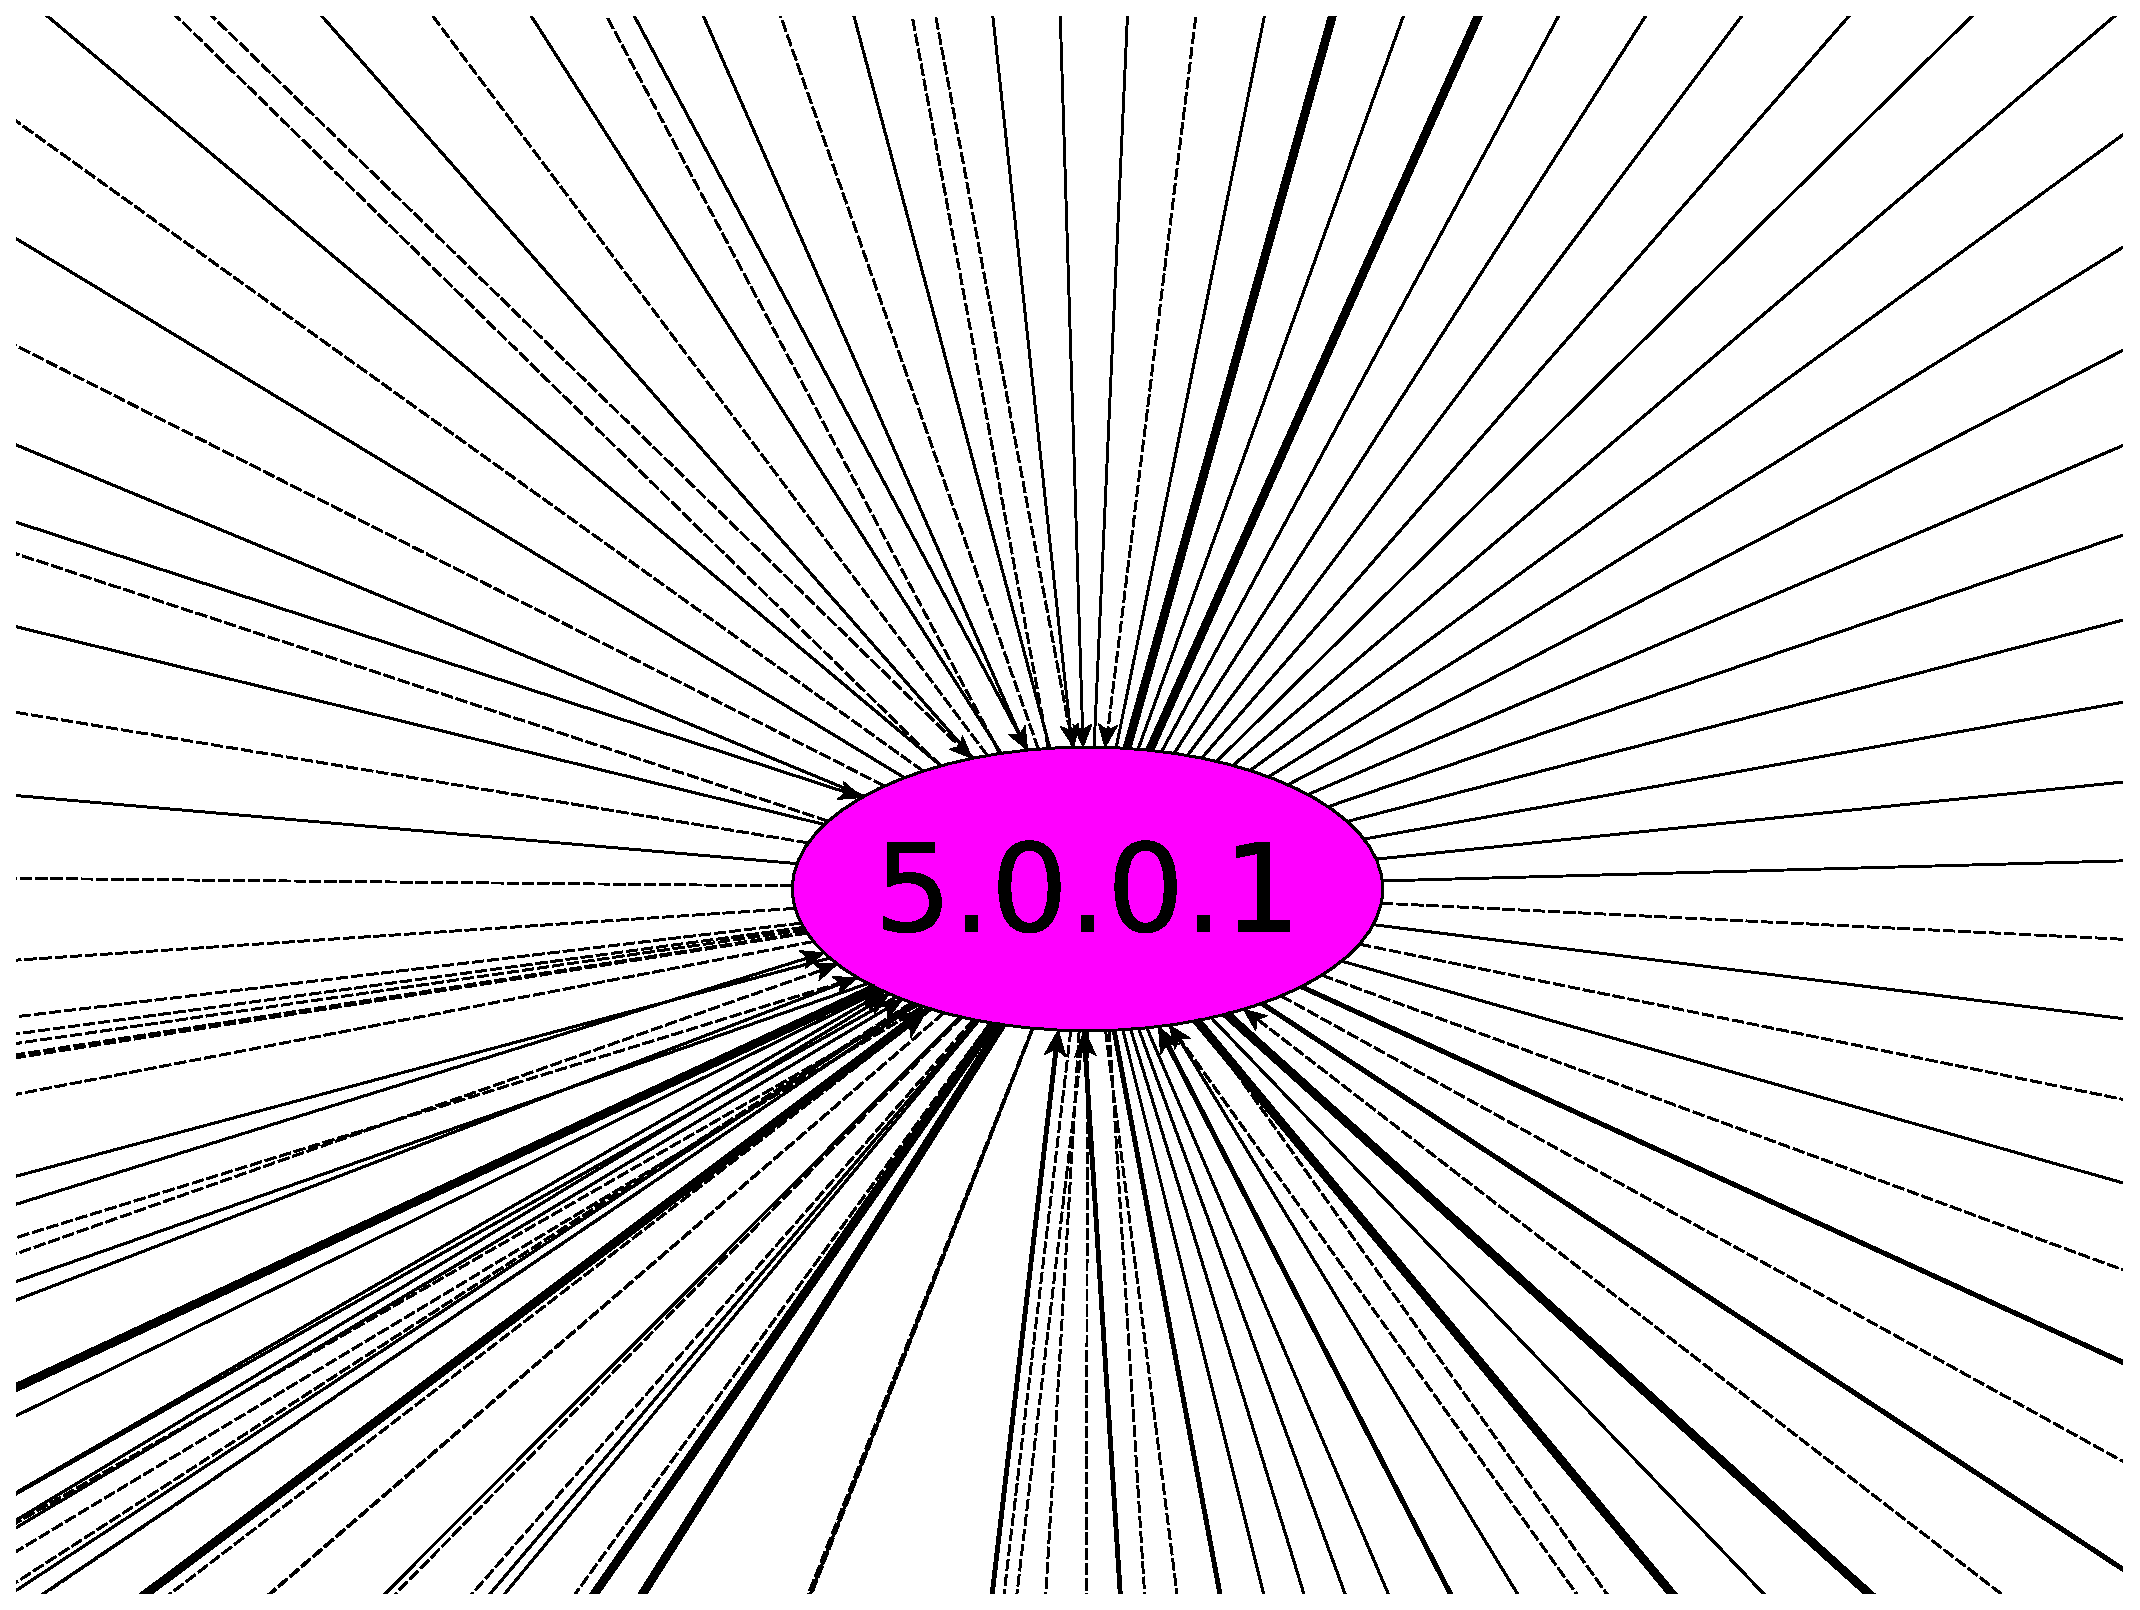
\includegraphics[width=0.5\textwidth]{img/graph/escenario_1/vlan10/vlan10_500toEnd_centro}
    \caption{Grafo VLAN \nameref{itm:vlan10} - Centro}
    \label{fig:vlan10_grafo_centro}
\end{figure}

\par Por \'ultimo, se observa una \textit{subregi\'on} en la zona izquierda donde varios
nodos parecer\'ieran estar env\'iandoso paquetes entre s\'i con bastante regularidad. A
\textit{prior\'i} estos parecer\'ian ser los nodos m\'as activos de la red durante el
transcurso de la semana. Se puede observar dicha zona en la figura \ref{fig:vlan10_grafo_inf}:

\begin{figure}
    \centering
    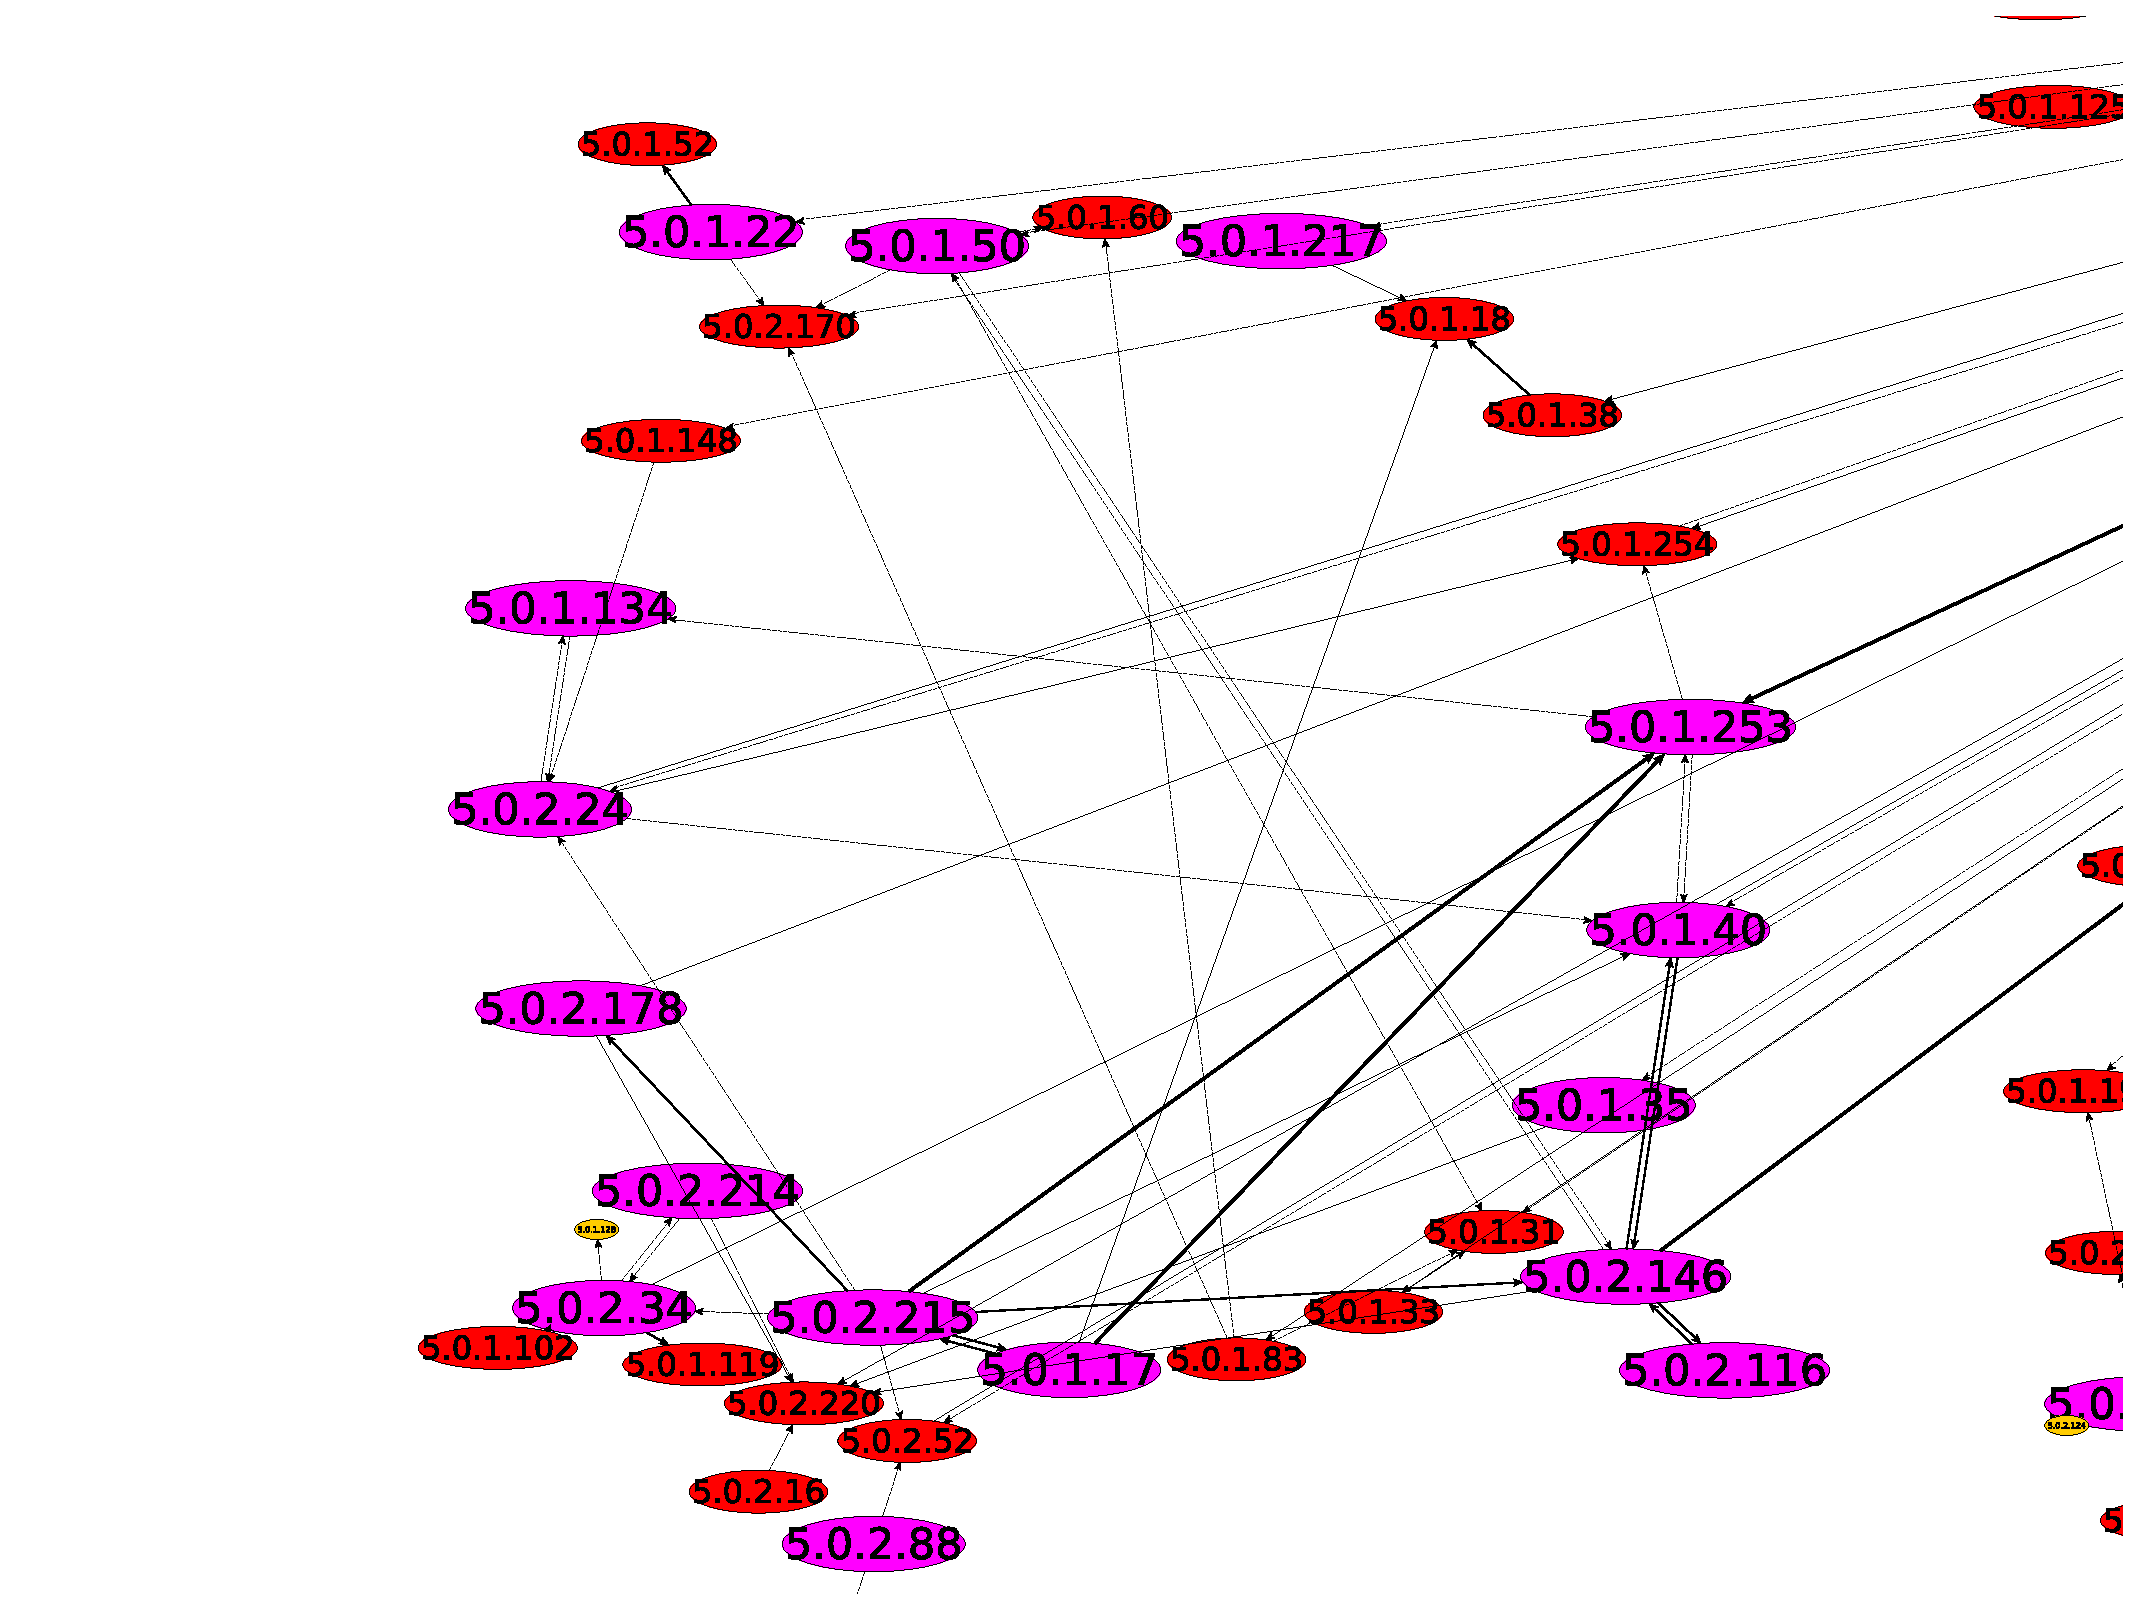
\includegraphics[width=0.5\textwidth]{img/graph/escenario_1/vlan10/vlan10_500toEnd_inf}
    \caption{Grafo VLAN \nameref{itm:vlan10} - Zona activa}
    \label{fig:vlan10_grafo_inf}
\end{figure}

\par En dicha regi\'on se puede ver que a pesar de la elevada actividad cruzada de paqutes
ARP entre los nodos, no hay nodo tan concurrido como el \textit{5.0.0.1}, el cual se
vi\'o en detalle hace tan solo unos momentos.


\subsubsection*{\underline{VLAN \nameref{itm:vlan10}: Conclusiones}}\label{subsubsec:vlan10_conclusiones}
\par Podemos concluir que claramente la direcci\'on \textit{5.0.0.1} es una
direcci\'on importante de la red. Se v\'io como aparece entre las direcciones con mayor
probabilidad tanto en la fuente de direcciones origen as\'i como destino, y se nota
en el grafo que es de entre los nodos con mayor probabilidad aquel que tiene la mayor
interacci\'on (en cuanto a cantidad) con el resto de los \textit{hosts} de la redes.

\par Este comportamiento es sumamente similar al comportamiento que tendr\'ia un equipo
encargado de \textit{routear} la red LAN hac\'ia otras redes, debido a la gran cantidad
de equipos que piden por su direcci\'on \textit{MAC} dentro de la VLAN.

\par Quiz\'as valga mencionar que de hecho hay otros nodos importantes en la red. Se
puede ver en la figura \ref{fig:vlan10_grafo_inf} como hay tres direcciones que se env\'ian
pedidos ARP con bastante frecuencia: \textit{5.0.1.253, 5.0.1.17, 5.0.2.15 y 5.0.246}.
No parecer\'ia ser casualidad que a todas estas IPs les haya correspondido el color
violeta en el grafo. Claramente la interaccion que tienen entre s\'i (m\'as all\'a de la
que tienen con los dem\'as nodos) parecer\'ia ser suficente, por las caracter\'isticas
de los ejes, para tener una alta probabilidad en ambas fuentes de s\'imbolos. Claramente
esto ser\'ia un dato de inter\'es para el administrador de la red, debido a que quiz\'as
estos equipos est\'an env\'iando paquetes broadcast en el dominio de colisi\'on sin
que haya necesidad.
